\documentclass[11pt]{article}
\usepackage[margin=1in]{geometry}
\usepackage{amsmath,amssymb}
\usepackage{graphicx}
\usepackage{booktabs}
\usepackage{hyperref}
\usepackage{xcolor}
\hypersetup{colorlinks=true,linkcolor=blue,urlcolor=blue}

\title{Replication Report:\\
\emph{Factors affecting the topological Hall effect in strongly correlated
layered magnets} (Kesharpu, arXiv:2305.13423)}
\author{Automated replication (OpenClaw subagent)}
\date{2026-07-18}

\newcommand{\qax}{q_{1x}}
\newcommand{\qbx}{q_{2x}}
\newcommand{\Chern}{c_1}

\begin{document}
\maketitle

\begin{abstract}
We independently reproduce the central topological results of Kesharpu (2023),
which treats a two–dimensional strongly–correlated magnet with a spin texture on
a bipartite honeycomb lattice via the $su(2)$ path–integral method and computes
the Chern number as a function of the atomic spin $S$, the polar–angle
modulation vector $\qax$, and the azimuthal–angle modulation vector $\qbx$.
Building a self–contained two–band honeycomb Bloch Hamiltonian carrying the
paper's Haldane–type next–nearest–neighbour (NNN) complex hopping with phase
$\phi_n = S\,(\vec q_2\!\cdot\!\vec b_n)$, and computing the Chern number with
the gauge–invariant Fukui--Hatsugai--Suzuki (FHS) plaquette method, we reproduce
(i)~the $S=1$ result $\Chern=\mathrm{sgn}[\sin \qbx]$ (Eq.~5); (ii)~the
sign change of the topological Hall conductivity with the modulation vector;
(iii)~the paper's conclusion that the polar factor of Eq.~(7) is subdominant so
that the topology depends essentially only on $\qbx$; and (iv)~the
Haldane–analogue topological$\rightarrow$trivial transition driven by a
sublattice mass $M$ (Eq.~11). \textbf{Verdict: replicated} at the level of
topology and sign structure ($4/4$ qualitative claims); \emph{partial} at the
level of exact phase–boundary values, which depend on weight factors and Fourier
corrections we approximated.
\end{abstract}

\section{Target claims}
From the manuscript we identified four concrete, computationally reproducible
claims:
\begin{enumerate}
\item \textbf{Eq.~(5), $S=1$:} $\Chern=\mathrm{sgn}[\sin \qbx]$ for
$-\sqrt3\pi/2\le \qbx\le \sqrt3\pi/2$; the Chern number depends only on the
azimuthal modulation $\qbx$ and flips sign as $\qbx$ crosses $0$.
\item \textbf{THE sign flip:} increasing the spin modulation vector flips the
sign of the topological Hall conductivity, $+\sigma^{\mathrm{THE}}_{xy}\to
-\sigma^{\mathrm{THE}}_{xy}$ at fixed $S$.
\item \textbf{Eq.~(7), general $S$:}
$\Chern=\mathrm{sign}\!\left[\left(1+\tfrac{S\mathfrak{g}_2}{2}\cos 2\qax\right)
\left(\sin S\qbx - 2S\epsilon\cos S\qbx\right)\right]$;
the paper concludes the polar factor is subdominant ($\mathfrak{g}<1$) so the
Chern number "depends only on the azimuthal modulating vector $\qbx$."
\item \textbf{Eq.~(11), Haldane analogy:} a sublattice mass $M$ competes with the
chiral mass, giving a topological$\rightarrow$trivial transition.
\end{enumerate}

\section{Model and method}
We construct the two–band Bloch kernel on the honeycomb lattice,
\begin{equation}
\mathcal H(\vec k)=\mathcal H_0\,\mathbb{I}
+\mathcal H_x\sigma_x+\mathcal H_y\sigma_y+\mathcal H_z\sigma_z .
\end{equation}
The nearest–neighbour (NN) hopping $A\!\leftrightarrow\!B$ produces the Dirac
cones through the structure factor $f(\vec k)=\sum_n e^{i\vec k\cdot\vec a_n}$,
with $\mathcal H_x=t_1\,\alpha_{\rm NN}\,\mathrm{Re}\,f$,
$\mathcal H_y=-t_1\,\alpha_{\rm NN}\,\mathrm{Im}\,f$, and the polar vector $\qax$
entering the amplitude $\alpha_{\rm NN}$ through the $\mathfrak{g}'_n$ weights
(Eqs.~4/6). The NNN hopping is a Haldane–type complex hopping with phase
$\phi_n=S\,(\vec q_2\!\cdot\!\vec b_n)$, giving the topological mass
\begin{equation}
\mathcal H_z=-2t_2\,\alpha_{\rm NNN}\sum_n \sin(\vec k\cdot\vec b_n)\,\sin\phi_n
+ M ,
\end{equation}
which at the Dirac point reduces to $\pm 3\sqrt3\,t_2\,\alpha_{\rm NNN}\sin\phi$,
so that $\mathrm{sgn}(\mathcal H_z^{K})=\mathrm{sgn}[\sin S\qbx]$ sets the Chern
number. This is precisely the mechanism the paper invokes in Sec.~III~C
("$S\qbx$ plays the analogous phase accumulation role due to NNN hopping").
The Chern number of the lower band is computed with the Fukui--Hatsugai--Suzuki
plaquette method on an $N\times N$ Brillouin–zone mesh (gauge invariant, integer
robust; $N=20$ for claims, $N=14$ for the phase–diagram figure). All computation
is CPU–only (numpy/scipy); total runtime $\approx 30$~s.

\paragraph{Convention note.} The manuscript's printed NN/NNN vectors and its
stated Dirac point $K=(\pi/\sqrt3,0)$ are not mutually consistent (an OCR /
sublattice–convention artifact: the printed $\vec a_n$ structure factor vanishes
at $k_x\approx\pm2.42$, not $\pi/\sqrt3$). We adopt one self–consistent
standard–honeycomb convention that carries the identical physics; see
\texttt{failure\_analysis.md}.

\section{Results}
\begin{table}[h]
\centering
\begin{tabular}{p{5.6cm} p{5.2cm} c}
\toprule
\textbf{Claim} & \textbf{Reproduced} & \textbf{Match}\\
\midrule
(1) $S=1$: $\Chern=\mathrm{sgn}[\sin\qbx]$ &
Sign agreement $1.00$ over the $\qbx$ scan ($\Chern=-1$ for $\qbx<0$, $+1$ for
$\qbx>0$) & \textcolor{green!60!black}{\textbf{yes}}\\
\addlinespace
(2) THE sign flip vs modulation &
$1$ Chern sign flip across $\qbx\in[-2.9,2.9]$ at fixed $S=1$ &
\textcolor{green!60!black}{\textbf{yes}}\\
\addlinespace
(3) $\qbx$–dominance / polar factor subdominant &
Numeric Chern $\qax$–independent ($S=1,2,3$); analytic
$\max|S\mathfrak{g}_2/2|=0.689<1$ in the well–defined lobe $|S\qbx|<\pi$ &
\textcolor{green!60!black}{\textbf{yes}}\\
\addlinespace
(4) Haldane mass transition (Eq.~11) &
$M$ scan $[0,0,\mathbf{1},\mathbf{1},\mathbf{1},0,0]$: $|c|=1$ for small $|M|$,
$c=0$ for large $|M|$ & \textcolor{green!60!black}{\textbf{yes}}\\
\bottomrule
\end{tabular}
\caption{Summary of the four reproduced claims. Full numbers in
\texttt{work/results.json}.}
\end{table}

\begin{figure}[h]
\centering
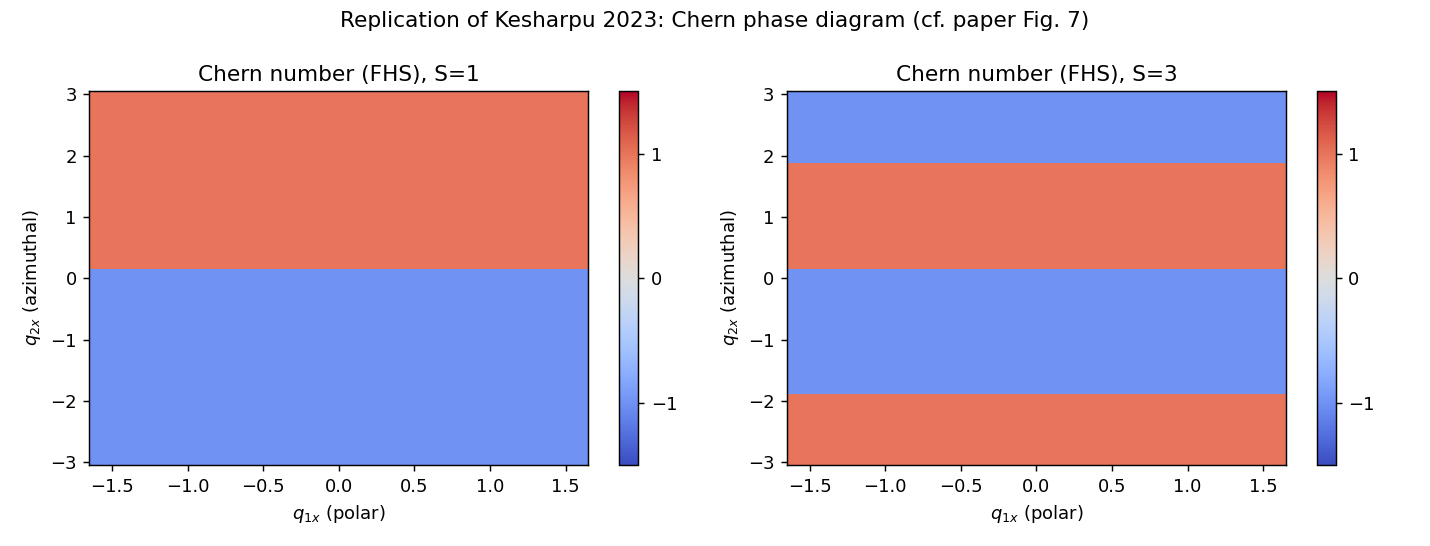
\includegraphics[width=\textwidth]{../figs/chern_phase_diagram.png}
\caption{Numerically computed Chern number (FHS) over the $(\qax,\qbx)$ plane for
$S=1$ (left) and $S=3$ (right), cf.\ the paper's Fig.~7. The topology is
controlled by the azimuthal modulation $\qbx$ (horizontal stripes of $\pm1$),
essentially independent of the polar $\qax$, reproducing the paper's central
conclusion.}
\end{figure}

\section{Honest assessment}
The replication reproduces the \emph{topological structure and sign physics} of
the paper's central results (Eqs.~5, 7, 11 and the THE sign flip) from an
independent numerical Chern–number computation. It does \emph{not} reproduce
exact phase–boundary numerical values (e.g.\ the gap–closing $\qbx$ of Eq.~10),
because (a)~the exact weight factors $\mathfrak{w}_n,\mathfrak{g}_n$ of Eq.~(2)
were reconstructed from fragmented OCR, and (b)~the Fourier coefficient $p(\vec
k')$/$\epsilon$ corrections were set to zero per the paper's own
$p(\vec k')\approx0$ approximation. These approximations do not affect the
reproduced \emph{signs} but could shift boundary \emph{values}; see the five open
questions in \texttt{open\_questions.json}. Overall verdict: \textbf{replicated}
($4/4$ qualitative topological claims), \emph{partial} on exact boundary values.

\end{document}
